% \begin{figure}[t]
%     \centering
%     \begin{subfigure}{0.5\textwidth}
%         \centering
%         \includegraphics[width=\textwidth]{fig/aurora-m-overall.pdf}
%         \caption{Overall performance compared to StarCoderBase and StarCoderPlus on multilingual code synthesis, and English (EN), Finnish (FI), Hindi (HI), Japanese (JA), and Vietnamese (VI) benchmarks.}
%         \label{fig:overall-results}
%     \end{subfigure}
%     \hfill
%     \begin{subfigure}{0.45\textwidth}
%         \label{data_distribution}
%         \centering
%         \includegraphics[width=\textwidth]{fig/output_file-1.pdf}
%         \caption{Data distribution of languages (EN, FI, HI, JA, VI), code and instructions in the training data ($\sim$435B tokens) used for the two-stage continual pretraining of the \system\ model. }
%         \label{fig:distribution}
%     \end{subfigure}
%     \vspace{-0.3em}
%     \caption{\textbf{Left}: Overall performance of {\system} on multilingual language and code benchmarks; \textbf{Right}: Pre-training data distribution over languages and code. }
%     \label{fig:intro}
% \end{figure}

% \begin{wrapfigure}{r}{0.5\textwidth}
%     \vspace{-15mm}
%   \begin{center}    \includegraphics[width=0.48\textwidth]{fig/aurora-m-overall.pdf}
%   \end{center}
%   \caption{}
%   \vspace{-8mm}
%   \label{fig:overall-results}
% \end{wrapfigure}

Large Language Models (LLMs) are fundamental tools in artificial intelligence, powering applications such as machine translation, text summarization, dialogue systems, and code generation. These LLMs are pre-trained on extensive text data to enhance downstream task-specific adaptation. However, the excessive computational expense of pretraining LLMs creates barriers to access, constraining wider development.

% Open-source efforts like BLOOM~\citep{scao2022bloom}, StarCoder \citep{li2023starcoder}, StarCoder-2 \citep{starcoder2}, Mistral \citep{jiang2023mistral} and OLMo \citep{groeneveld2024olmo,soldaini2024dolma} have emerged to democratize access to pre-trained LLMs. These projects play a vital role in fostering innovation and enabling researchers and developers to build upon existing advancements. However, several key challenges remain in the realm of open-source LLM development. Firstly,  several studies \citep{bang2023multitask, jiao2023chatgpt, hendy2023good, zhu2023multilingual, huang2023languages} highlighted how LLMs still struggle when dealing with non-English texts, especially in low-resource or extremely low-resource languages, as their training data is primarily dominated by English. For instance, \cite{brown2020language} stated that the English language accounts for 93\% of the total composition of GPT-3's training data. Hence, to further democratize LLMs and minimize performance gaps across different languages, it is crucial to promote the development of multilingual models~\citep{chai2023ernie}. Secondly, continual pre-training, a technique where a pre-trained model is further trained on new data distributions to enhance its capabilities, presents a significant challenge. While this approach offers the potential to improve performance, it often leads to catastrophic forgetting, where the model loses previously learned abilities. This phenomenon becomes even more concerning when considering the continual pre-training of models on a multitude of grammatically and lexically diverse languages. Finally, ensuring compliance with recent regulations mandating safe and secure AI development practices is another critical aspect that is often not addressed in open-source LLM development.

Open-source initiatives such as \textsc{Bloom} \citep{scao2022bloom}, \textsc{StarCoder} \citep{li2023starcoder}, \textsc{StarCoder-2} \citep{starcoder2}, \textsc{Pythia} \citep{biderman2023pythia}, and \textsc{OLMo} \citep{groeneveld2024olmo,soldaini2024dolma} have emerged to democratize access to pre-trained LLMs. These initiatives stimulate innovation, allowing researchers and developers to leverage existing advancements. However, despite their contributions, several significant challenges persist in the domain of open-source LLM development.

Primarily, several studies \citep{bang2023multitask, jiao2023chatgpt, hendy2023good, huang2023languages} have underscored the ongoing struggle of LLMs with non-English texts, particularly in low- or extremely low-resource languages.  Given that the training data predominantly consists of English, as noted for instance by \citet{brown2020language} who reported that English accounts for 93\% of GPT-3's training corpus, there is a pressing need to promote the development of multilingual models to democratize LLMs and alleviate performance disparities across different languages \citep{chai2023ernie}. Secondly, continual pretraining -- a technique involving further updating pretrained models on new data distributions to enhance their capabilities \citep{gupta2023continual, fujii2024continual} -- poses a significant challenge. While this approach could potentially enable life-long learning of large language models, it often leads to catastrophic forgetting, where the model loses previously acquired knowledge. This challenge is exacerbated when considering the continual pretraining of models across a diverse array of grammatical and lexical structures. Lastly, ensuring compliance with recent regulations mandating safe and secure AI development practices represents another critical aspect often overlooked in open-source LLM development, specifically, for multilingual models.


This paper presents \textcolor{violet}{\system}, a novel open-source multilingual Large Language Model (LLM) with 15 billion parameters, tailored to address the aforementioned limitations. \system\ is designed to cater to five linguistically diverse languages: English, Finnish, Hindi, Japanese, Vietnamese, with a mix of code data. \system\ is continually pretrained from the \textsc{StarCoderPlus} model~\citep{li2023starcoder} on an extensive dataset comprising 435 billion tokens, resulting in a total training token count of an impressive 2 trillion tokens. This rigorous pretraining regimen equips \system\ with a comprehensive understanding of diverse languages and code. Moreover, safety is a fundamental design principle of \system. It stands out as the first open-source multilingual LLM fine-tuned on a comprehensive collection of human-reviewed safety instructions addressing concerns in the Biden-Harris Executive
Order on Safe, Secure, and Trustworthy Development and Use of Artificial Intelligence~\citep{whitehouse2023fact}. This fine-tuning process not only addresses conventional red-teaming concerns~\citep{ganguli2022red,perez2022red} aimed at testing system vulnerabilities, but also aligns with the specific safety and security guidelines outlined in the Order.


% To comprehensively evaluate \system's effectiveness, we conduct a rigorous examination across a broad range of tasks spanning multiple domains and languages.  Our evaluations are designed to assess \system's ability to maintain previously learned knowledge while acquiring new capabilities through continual pre-training. We demonstrate that \system\ successfully avoids catastrophic forgetting on English and coding tasks.  Moreover, we benchmark \system\ against state-of-the-art multilingual models, showcasing its competitive performance in these settings.  Additionally, safety evaluations are conducted to analyze \system's propensity for generating unwanted or potentially illegal content.  The results from these evaluations confirm that \system\ prioritizes safety and adheres to responsible AI development practices.  

To comprehensively evaluate \system's efficacy, we conduct a rigorous examination across a diverse spectrum of tasks spanning various domains and languages. Our evaluations aim to gauge \system's capacity to retain previously learned knowledge while acquiring new capabilities through continual pretraining. We demonstrate that \system\ successfully avoids catastrophic forgetting on English and coding tasks. Furthermore, we benchmark \system\ against state-of-the-art multilingual models, showcasing its competitive performance in these settings. Additionally, safety evaluations are conducted to scrutinize \system's tendency to generate undesired or potentially illicit content. The findings from these assessments affirm \system's commitment to safety and the adherence to responsible AI development practices.


\begin{figure*}[t]
\begin{center}
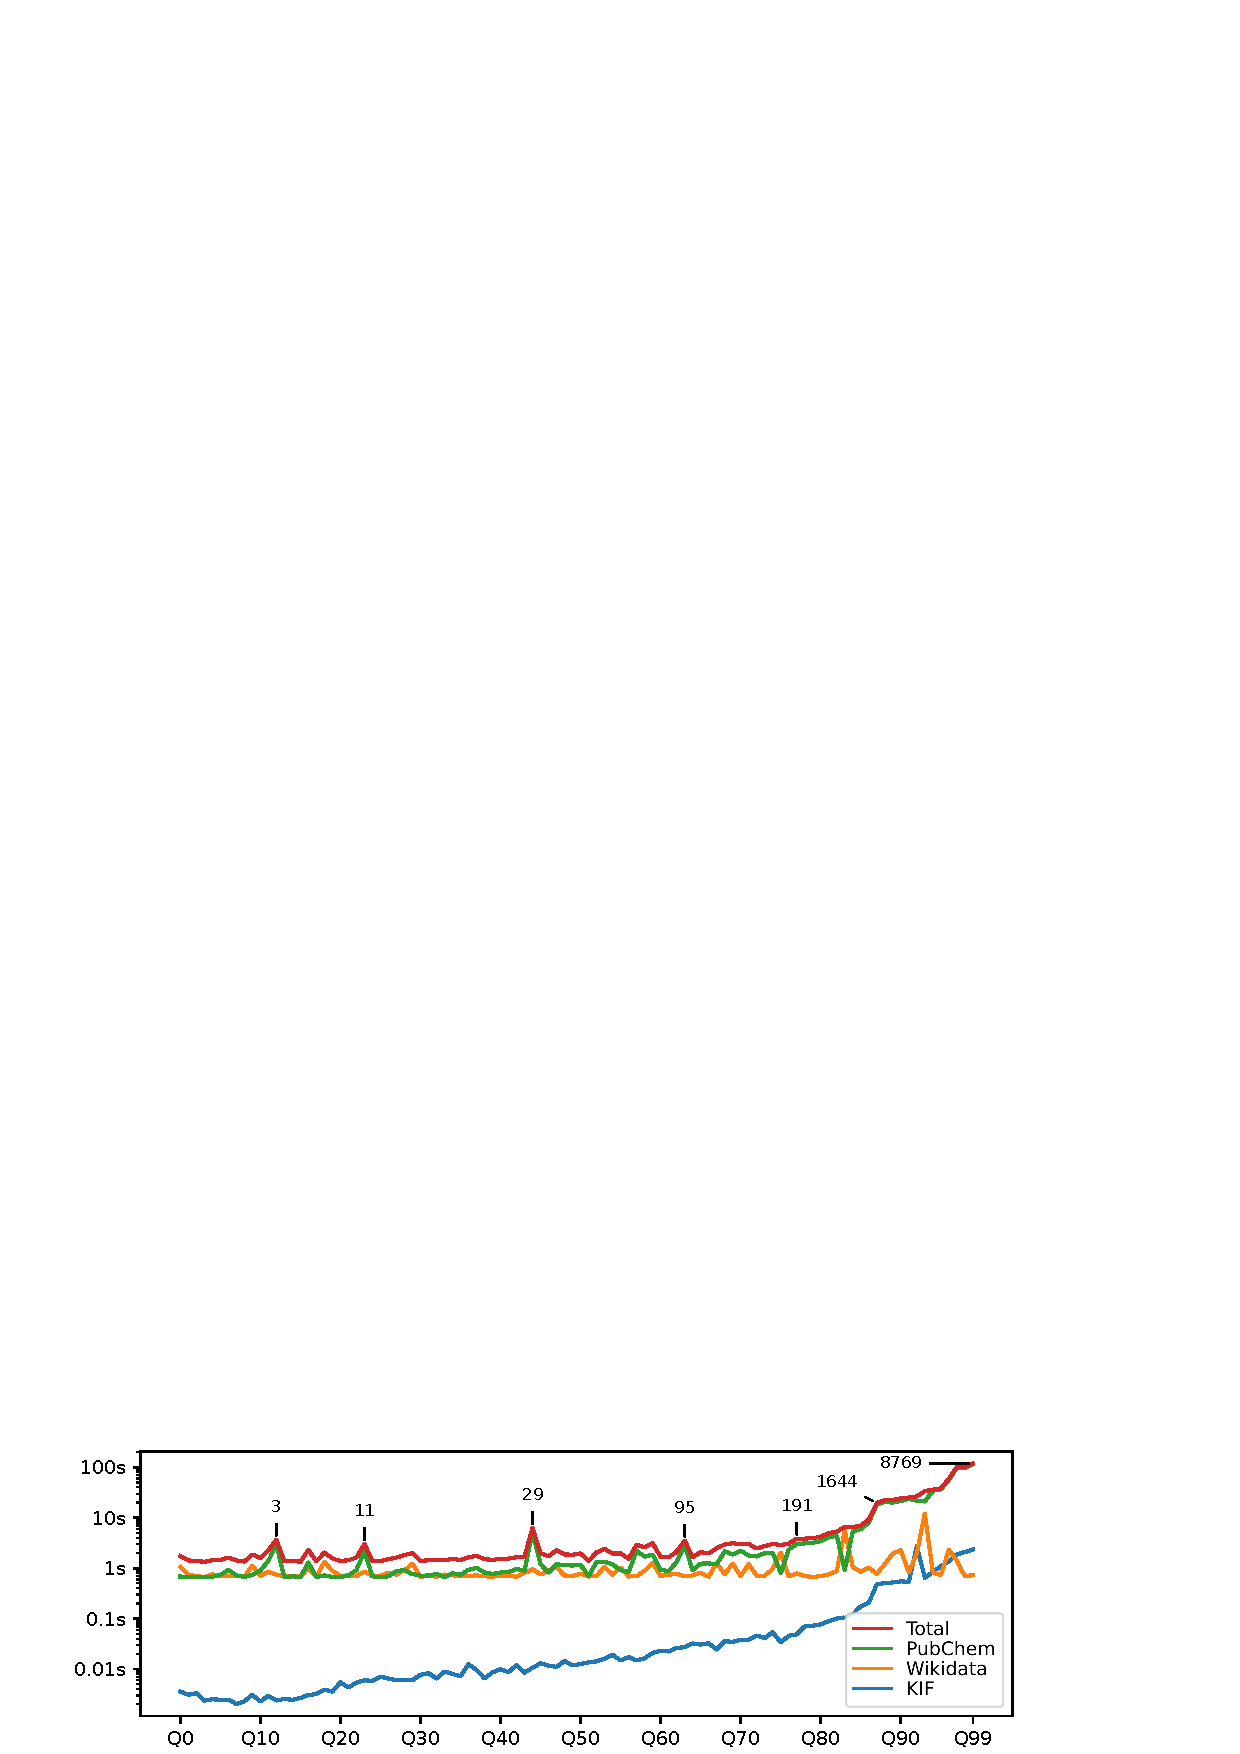
\includegraphics[width=\textwidth]{fig/plot.pdf}
\end{center}
\vspace{-8mm}
\caption{Comparison of overall performance between \textcolor{violet}{\system}-redteamed and its predecessors, \textsc{StarCoderBase} and \textsc{StarCoderPlus}, across diverse code and multilingual language evaluation benchmarks. Pass@1 performance averages for code benchmarks are reported. For natural language evaluations, 0-shot accuracy averages are reported for languages other than English and Japanese. English evaluation is 8-shot, while Japanese evaluation uses a combination of 4-shot and 1-shot.}
\vspace{-4.2mm}
\label{fig:overall}
\end{figure*} 

% In recognition of the importance of fostering responsible development within the LLM community, we are publicly releasing \system\ and its variants. This will enable researchers and developers to leverage \system's capabilities while adhering to best practices in safe and secure AI development.



% Large Language Models (LLMs) exhibit remarkable abilities in text understanding and generation, as demonstrated by the OpenAI’s GPT model family \citep{brown2020language}. However, despite their impressive performance, the specific training and architectural aspects of these models tend to remain opaque, posing challenges for research and open science advancements in this domain. In contrast, advocating for open-source LLMs can enhance innovation, accessibility, and transparency. 

% Additionally, several studies \citep{bang2023multitask, jiao2023chatgpt, hendy2023good, zhu2023multilingual, huang2023languages} highlighted how LLMs still struggle when dealing with non-English texts, especially in low-resource or extremely low-resource languages, as their training data is primarily dominated by English. For instance, \cite{brown2020language} stated that the English language accounts for 93\% of the total composition of GPT-3’s training data. Hence, to further democratize LLMs and minimize performance gaps across different languages, it is crucial to promote the development of multilingual models~\citep{chai2023ernie}.

% In this work, inspired by pioneering efforts in open-sourcing LLMs \citep{touvron2023llama, almazrouei2023falcon, jiang2023mistral}, and motivated by the above-mentioned limitations, we introduce \system\, a multilingual, multidomain, and multimodal model consisting of 15B parameters. It is a Starcoderplus-based \citep{li2023starcoder} model continually pretrained on $\sim$435B domain-specific tokens on top of the $\sim$1.5T tokens from the Stack \citep{Kocetkov2022TheStack}, Refined Web \citep{refinedweb}, Red Pajama 1 \citep{together2023redpajama}, and Pile \citep{gao2020pile}. It is specifically designed to cover a vast array of domains -- including chemical SMILEs formula, financial data, legal contracts, political debates, climate change data, ABC music notations, coding, and math -- as well as multiple languages, i.e.~English, Finnish, Hindi, Japanese, and Vietnamese. Notably, as depicted in Figure \ref{fig:distribution}, only 37\% of the data utilized for the continuous pretraining of \system\ corresponds to English text.

% Moreover, \system\ is further trained on thousands of human-reviewed, red-teaming instructions to address general safety concerns, and more specifically the concerns in the Biden-Harris Executive Order on AI.\footnote{\href{https://www.whitehouse.gov/briefing-room/statements-releases/2023/10/30/fact-sheet-president-biden-issues-executive-order-on-safe-secure-and-trustworthy-artificial-intelligence/}{US Executive Order on Safe, Secure, and Trustworthy Artificial Intelligence}}

Our contributions can be summarized as follows.
\begin{itemize}
    \vspace{-0.2em}
    %\itemsep-0.3em 
    \item We introduce \textcolor{violet}{\system}, a new 15B continually pretrained red-teamed multilingual LLM built on top of the StarCoderPlus model~\citep{li2023starcoder}.
    \item We develop a two-stage curriculum of continual pretraining consisting of \textbf{Continual Auxiliary Pretraining} (CAP) and \textbf{Continual Alignment Tuning} (CAT) aimed at maximizing adaptation, minimizing catastrophic forgetting, and aligning \system\ with safety objectives. 
    \item We extensively evaluate \system\ across various tasks in different domains and languages, demonstrating its superior performance in multilingual settings while retaining competitive performance in English and coding.
    \item We construct a new red-teaming dataset, named ``\text{The Biden-Harris Redteam Dataset},'' tailored to address concerns outlined in the Executive Order along with typical safety concerns. We then fine-tune \system\ on this dataset and evaluate on several safety benchmarks.
    \item We show the influence of scaling the total training tokens on various multilingual and code evaluation tasks.
    \vspace{-0.2em}
\end{itemize}
% We hope that our work will provide a stepping stone for further studies on the responsible development of open-source, multilingual LLMs and contribute to their democratization.

%It was developed by an open-source and open-science community of volunteers spanning several international institutions. The development began as a grassroots effort and stretched over 9 months and produced a model that is both performing and proficient in multiple domains and languages.

%However we need a mechanism to train more capable models in an efficient and modular way.
% s

%Many models are good for English and code, but not many for other languages. We show that it is possible to efficiently create expert models and transfer knowledge between multiple languages, and that the models can handle long contexts.

%Our method is to perform continued pretraining on massive and diverse data on a mixture of languages, domain and code data and then applying cBTM LoRAs on specific subsets of the data that has been converted into instruction format.



% \begin{figure}[!t]
% \begin{center}
% \includegraphics[width=0.7\textwidth]{img/dist_2.png}
% \end{center}
% \caption{Distribution of languages and code in the training data ($\sim$435B tokens) used for the continual pretraining of the \system\ model. \color{red}{Liangyu: do we have this img in pdf? actually we should present all the figures in pdf.}}
% \label{fig:distribution}
% \end{figure}